\documentclass[11pt,a4paper]{article}
\usepackage[T1]{fontenc}
\usepackage[utf8]{inputenc}
\usepackage{lmodern}
\usepackage{textcomp}
\usepackage[left=1.8cm,right=1.8cm,top=2.3cm,bottom=2.2cm,headheight=14pt,headsep=8pt]{geometry}
\usepackage{multicol}
\usepackage{xcolor}
\usepackage{fancyhdr}
\usepackage{graphicx}
\usepackage{array}
\usepackage{amsmath,amssymb}
\usepackage{setspace}
\usepackage{longtable}
\graphicspath{{../}}
\definecolor{ygreen}{RGB}{46,139,87}
\renewcommand{\normalsize}{\fontsize{10.9}{13.4}\selectfont}
\renewcommand{\familydefault}{\rmdefault}
\setlength{\parindent}{0pt}
\setlength{\columnsep}{0.8cm}
\setlength{\columnseprule}{0.4pt}
\setlength{\multicolsep}{3pt plus 1pt minus 1pt}
\renewcommand{\textsubscript}[1]{\ensuremath{_{\text{\fontsize{8}{8}\selectfont #1}}}}
\renewcommand{\textsuperscript}[1]{\ensuremath{^{\text{\fontsize{8}{8}\selectfont #1}}}}
\newcommand{\diqqat}[1]{\par\smallskip\noindent\textbf{Diqqat!} #1\par\medskip}
\newcommand{\javob}{\par\smallskip\noindent\textbf{Javob:} \rule[-2pt]{7.5cm}{0.4pt}\par\smallskip\noindent\textbf{Diqqat!} Javobingizni javoblar varaqasiga ko`chirib yozing.\par\medskip}
\pagestyle{fancy}
\fancyhf{}
\renewcommand{\headrulewidth}{0.4pt}
\fancyhead[L]{\textit{Milliy sertifikat 2026. Kimyo}}
\fancyhead[R]{13-variant}
\fancyfoot[L]{\fontsize{8}{9}\selectfont \textcopyright{} Colba maktabi, 2026}
\fancyfoot[C]{\thepage}
\fancypagestyle{first}{\fancyhf{}\renewcommand{\headrulewidth}{0pt}\fancyfoot[L]{\fontsize{8}{9}\selectfont \textcopyright{} Colba maktabi, 2026}\fancyfoot[C]{\thepage}}
\begin{document}
\normalsize
\thispagestyle{first}
\noindent\fcolorbox{ygreen}{white}{\parbox{\dimexpr\linewidth-2\fboxsep-2\fboxrule\relax}{%
\textbf{\fontsize{13}{15}\selectfont Nazorat testi}\ \textit{\fontsize{10}{12}\selectfont $\cdot$ Aralash test $\cdot$ 13-variant}\hfill
\begin{tabular}[t]{@{}r@{}}\textit{Milliy sertifikat 2026. Kimyo}\\ \textbf{\textit{\fontsize{8}{9}\selectfont Vaqt:}} \textit{\fontsize{10}{12}\selectfont 180 daqiqa}\end{tabular}}}
\par\medskip
\noindent\textit{Davriy jadvaldan foydalanish mumkin.}
\par\medskip
\begin{multicols}{2}
\noindent\textbf{1.} CO + Cl\textsubscript{2} $\rightleftarrows$ COCl\textsubscript{2} reaksiyasi 2 l hajmli idishda o`tkazildi. Ma'lumotlar jadvalda berilgan:
\begin{center}
\renewcommand{\arraystretch}{1.15}
\begin{tabular}{|c|c|c|c|}\hline
\textbf{Modda} & \textbf{CO} & \textbf{Cl\textsubscript{2}} & \textbf{COCl\textsubscript{2}} \\ \hline
Boshlang`ich, mol & 6 & 3 & 0 \\ \hline
Muvozanatda, mol & --- & --- & 0,5 \\ \hline
\end{tabular}
\end{center}
Muvozanat \textbf{konstantasini (K) hisoblang.}

\noindent A)~\textsl{0,073} \hfill B)~\textsl{0,145} \hfill C)~\textsl{0,036} \hfill D)~\textsl{13,75}\par
\vspace{4pt}
\noindent\textbf{2.} CO + Cl\textsubscript{2} $\rightleftarrows$ COCl\textsubscript{2} reaksiyasi 1 l hajmli idishda o`tkazildi. Ma'lumotlar jadvalda berilgan:
\begin{center}
\renewcommand{\arraystretch}{1.15}
\begin{tabular}{|c|c|c|c|}\hline
\textbf{Modda} & \textbf{CO} & \textbf{Cl\textsubscript{2}} & \textbf{COCl\textsubscript{2}} \\ \hline
Boshlang`ich, mol & 6 & 6 & 0 \\ \hline
Muvozanatda, mol & --- & --- & 1 \\ \hline
\end{tabular}
\end{center}
CO ning necha foizi reaksiyaga \textbf{kirishganini aniqlang.}

\noindent A)~\textsl{8,3} \hfill B)~\textsl{16,7} \hfill C)~\textsl{25} \hfill D)~\textsl{83,3}\par
\vspace{4pt}
\noindent\textbf{3.} N\textsubscript{2} + 3H\textsubscript{2} $\rightleftarrows$ 2NH\textsubscript{3} reaksiyada muvozanat holatida [N\textsubscript{2}] = 0,5, [H\textsubscript{2}] = 2, [NH\textsubscript{3}] = 2 mol/l. Muvozanat \textbf{konstantasini (K) hisoblang.}

\noindent A)~\textsl{2} \hfill B)~\textsl{0,5} \hfill C)~\textsl{1} \hfill D)~\textsl{1,6}\par
\vspace{4pt}
\noindent\textbf{4.} Qaysi juftliklarda reaksiya bormaydi? 1) Mg va FeSO\textsubscript{4}; 2) Cu va AgNO\textsubscript{3}; 3) Fe va MgCl\textsubscript{2}; 4) Cu va ZnSO\textsubscript{4}

\noindent A)~\textsl{4} \hfill B)~\textsl{3, 4} \hfill C)~\textsl{1, 2, 3} \hfill D)~\textsl{1, 3}\par
\vspace{4pt}
\noindent\textbf{5.} N\textsubscript{2} gazining 27 \textdegree{}C va 4 atm bosimdagi \textbf{zichligini (g/l) aniqlang.} (R = 0,082 l$\cdot$atm/(mol$\cdot$K))

\noindent A)~\textsl{9,11} \hfill B)~\textsl{2,28} \hfill C)~\textsl{4,55} \hfill D)~\textsl{1,25}\par
\vspace{4pt}
\noindent\textbf{6.} NaCl eritmasi inert elektrodlar yordamida 10 A tok kuchi bilan 9650 s elektroliz qilindi. Katodda ajralgan H\textsubscript{2} massasi (g) \textbf{ni toping.}

\noindent A)~\textsl{1} \hfill B)~\textsl{2} \hfill C)~\textsl{0,5} \hfill D)~\textsl{1,5}\par
\vspace{4pt}
\noindent\textbf{7.} A elementi atomining ketma-ket ionlanish energiyalari diagrammada berilgan.
\begin{center}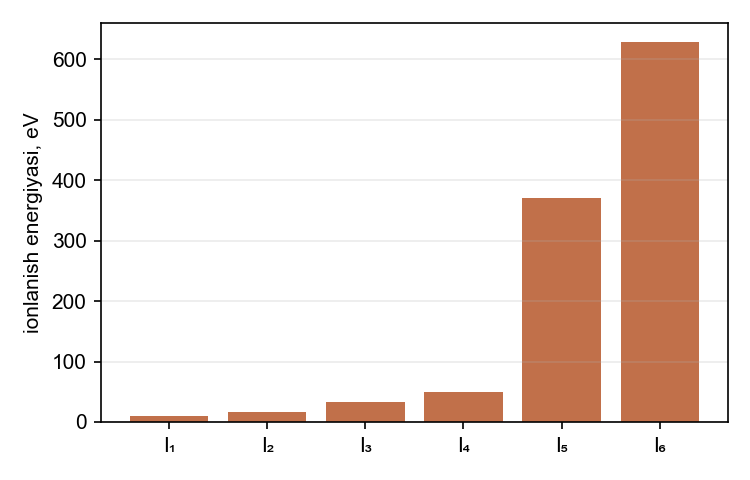
\includegraphics[width=0.86\linewidth]{rasmlar/gen/ie_v13_0.png}\end{center}
A elementi davriy jadvalning qaysi guruhida joylashgan?

\noindent\begin{tabular}{@{}p{0.47\linewidth}@{}p{0.47\linewidth}@{}}
A)~\textsl{IA guruh} & B)~\textsl{IIA guruh} \\
C)~\textsl{IIIA guruh} & D)~\textsl{IVA guruh} \\
\end{tabular}\par
\vspace{4pt}
\noindent\textbf{8.} Quyidagi tuzlarning qaysilari suvli eritmasi neytral muhitga ega? 1) Na\textsubscript{2}SO\textsubscript{4}; 2) CH\textsubscript{3}COONa; 3) NH\textsubscript{4}Cl; 4) KNO\textsubscript{3}

\noindent A)~\textsl{1, 4} \hfill B)~\textsl{1, 2, 3} \hfill C)~\textsl{1, 3} \hfill D)~\textsl{3}\par
\vspace{4pt}
\noindent\textbf{9.} Zichligi 1,4 g/ml bo`lgan 30\% li HCl eritmasining molyar \textbf{konsentratsiyasini (mol/l) aniqlang.}

\noindent A)~\textsl{1,15} \hfill B)~\textsl{23,01} \hfill C)~\textsl{11,51} \hfill D)~\textsl{8,22}\par
\vspace{4pt}
\noindent\textbf{10.} 8 g NaOH ni to`liq neytrallash uchun 7,3 g HCl sarflandi. HCl ning ekvivalent \textbf{massasini (g/mol) aniqlang.}

\noindent A)~\textsl{36,5} \hfill B)~\textsl{73} \hfill C)~\textsl{18,25} \hfill D)~\textsl{7,3}\par
\vspace{4pt}
\noindent\textbf{11.} C\textsubscript{6}H\textsubscript{5}OH molekulasidagi $\sigma$ va $\pi$ bog`lar \textbf{sonini aniqlang.}

\noindent A)~\textsl{12 va 3} \hfill B)~\textsl{13 va 4} \hfill C)~\textsl{14 va 3} \hfill D)~\textsl{13 va 3}\par
\vspace{4pt}
\noindent\textbf{12.} CuCl\textsubscript{2} ning suvli eritmasi inert elektrodlar bilan elektroliz qilinganda qaysi moddalar ajraladi?

\noindent\begin{tabular}{@{}p{0.47\linewidth}@{}p{0.47\linewidth}@{}}
A)~\textsl{Cu va Cl\textsubscript{2}} & B)~\textsl{Zn, H\textsubscript{2} va O\textsubscript{2}} \\
C)~\textsl{Ag va O\textsubscript{2}} & D)~\textsl{H\textsubscript{2}, Cl\textsubscript{2} va NaOH} \\
\end{tabular}\par
\vspace{4pt}
\noindent\textbf{13.} Alyuminiy (\textit{Z} = 13) atomining tashqi energetik pog`onasidagi elektronlar \textbf{sonini aniqlang.}

\noindent A)~\textsl{4} \hfill B)~\textsl{2} \hfill C)~\textsl{3} \hfill D)~\textsl{5}\par
\vspace{4pt}
\noindent\textbf{14.} 2Mg + CO\textsubscript{2} $\to$ 2MgO + C reaksiyasida 4,4 g CO\textsubscript{2} ishtirok etdi. C \textbf{miqdorini (mol) toping.}

\noindent A)~\textsl{0,2} \hfill B)~\textsl{0,05} \hfill C)~\textsl{0,15} \hfill D)~\textsl{0,1}\par
\vspace{4pt}
\noindent\textbf{15.} Reaksiya tenglamasi: H\textsubscript{2} + Cl\textsubscript{2} $\to$ 2HCl. Reaksiyaga 0,5 g H\textsubscript{2} kirishdi. HCl \textbf{hajmini (l, n.sh.) hisoblang.}

\noindent A)~\textsl{2,8} \hfill B)~\textsl{11,2} \hfill C)~\textsl{22,4} \hfill D)~\textsl{5,6}\par
\vspace{4pt}
\noindent\textbf{16.} Ishqoriy metallar haqida qaysi fikrlar to`g`ri? 1) Litiy eng yengil metall; 2) Natriy suv bilan reaksiyada H\textsubscript{2} va NaOH hosil qiladi; 3) Natriyning olinishi suyuqlanma NaCl elektrolizi bilan; 4) Natriy atomining tashqi qavatida 2 ta elektron bor

\noindent A)~\textsl{1, 3} \hfill B)~\textsl{1, 4} \hfill C)~\textsl{1, 2} \hfill D)~\textsl{1, 2, 3}\par
\vspace{4pt}
\noindent\textbf{17.} Alyuminiy va magniy dan iborat 10,5 g aralashma mo`l NaOH eritmasida eritildi. Ajralgan gazning \textbf{hajmini (l, n.sh.) aniqlang} (magniy ishqor bilan reaksiyaga kirishmaydi).

\noindent A)~\textsl{20,16} \hfill B)~\textsl{5,04} \hfill C)~\textsl{10,08} \hfill D)~\textsl{8,71}\par
\vspace{4pt}
\noindent\textbf{18.} D-metallar va ularning birikmalari haqida qaysi fikrlar to`g`ri? 1) Fe(OH)\textsubscript{2} havoda qo`ng`ir rangga o`tadi; 2) Zn(OH)\textsubscript{2} amfoter xossaga ega; 3) Mis nam havoda (CuOH)\textsubscript{2}CO\textsubscript{3} qoplamasi bilan qoplanadi; 4) Temir sovuq konsentrlangan HNO\textsubscript{3} da passivlanadi

\noindent\begin{tabular}{@{}p{0.47\linewidth}@{}p{0.47\linewidth}@{}}
A)~\textsl{1, 2, 4} & B)~\textsl{1, 2, 3, 4} \\
C)~\textsl{1, 3, 4} & D)~\textsl{2, 3, 4} \\
\end{tabular}\par
\vspace{4pt}
\noindent\textbf{19.} Reaksiya tenglamasi: MgCl\textsubscript{2} + Na\textsubscript{2}CO\textsubscript{3} $\to$ MgCO\textsubscript{3} + 2NaCl. Reaksiyaga 47,5 g MgCl\textsubscript{2} kirishdi. MgCO\textsubscript{3} \textbf{massasini (g) hisoblang.}

\noindent A)~\textsl{84} \hfill B)~\textsl{42} \hfill C)~\textsl{21} \hfill D)~\textsl{63}\par
\vspace{4pt}
\noindent\textbf{20.} Alkanlar va sikloalkanlar haqida qaysi fikrlar to`g`ri? 1) Sikloalkanlarning umumiy formulasi CnH\textsubscript{2}n; 2) Metanning katalitik oksidlanishidan formaldegid olinadi; 3) Metan suvda yaxshi eriydi; 4) Propan odatiy sharoitda gaz

\noindent A)~\textsl{1, 3, 4} \hfill B)~\textsl{1, 3} \hfill C)~\textsl{1, 2, 4} \hfill D)~\textsl{2, 4}\par
\vspace{4pt}
\noindent\textbf{21.} Etilen va asetilendan iborat 5,4 g aralashma mo`l bromli suv bilan to`liq reaksiyaga kirishdi. Sarflangan brom \textbf{massasini (g) aniqlang.}

\noindent A)~\textsl{96} \hfill B)~\textsl{48} \hfill C)~\textsl{24} \hfill D)~\textsl{32}\par
\vspace{4pt}
\noindent\textbf{22.} 64 g CaC\textsubscript{2} dan quyidagi ikki bosqichda C\textsubscript{6}H\textsubscript{6} olinadi: 1) CaC\textsubscript{2} + 2H\textsubscript{2}O $\to$ C\textsubscript{2}H\textsubscript{2} + Ca(OH)\textsubscript{2} (unum 50\%); 2) 3C\textsubscript{2}H\textsubscript{2} $\to$ C\textsubscript{6}H\textsubscript{6} (unum 90\%). Oxirgi mahsulot C\textsubscript{6}H\textsubscript{6} ning \textbf{massasini (g) toping.}

\noindent A)~\textsl{23,4} \hfill B)~\textsl{13} \hfill C)~\textsl{26} \hfill D)~\textsl{11,7}\par
\vspace{4pt}
\noindent\textbf{23.} Rasmda tasvirlangan molekuladagi sp\textsuperscript{3}-gibridlangan uglerod atomlari \textbf{sonini aniqlang.}
\begin{center}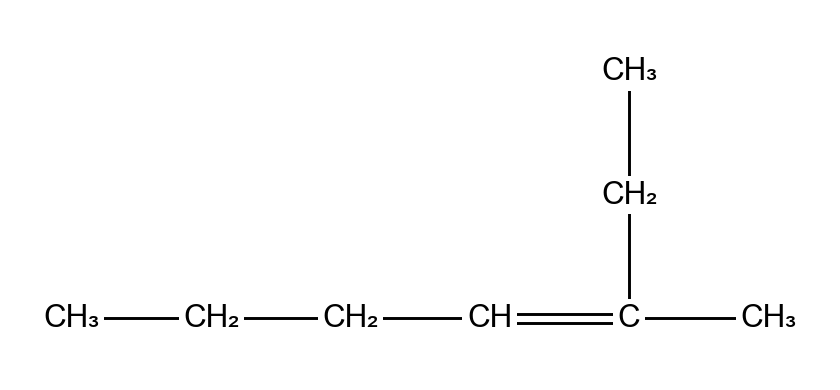
\includegraphics[width=0.86\linewidth]{rasmlar/gen/struct_16944700_887.png}\end{center}

\noindent A)~\textsl{6} \hfill B)~\textsl{7} \hfill C)~\textsl{5} \hfill D)~\textsl{8}\par
\vspace{4pt}
\noindent\textbf{24.} 22 g CH\textsubscript{3}CHO dan quyidagi ikki bosqichda (CH\textsubscript{3}COO)\textsubscript{2}Zn olinadi: 1) CH\textsubscript{3}CHO + 2Cu(OH)\textsubscript{2} $\to$ CH\textsubscript{3}COOH + Cu\textsubscript{2}O + 2H\textsubscript{2}O (unum 90\%); 2) 2CH\textsubscript{3}COOH + Zn $\to$ (CH\textsubscript{3}COO)\textsubscript{2}Zn + H\textsubscript{2} (unum 90\%). Oxirgi mahsulot (CH\textsubscript{3}COO)\textsubscript{2}Zn ning \textbf{massasini (g) toping.}

\noindent A)~\textsl{41,18} \hfill B)~\textsl{37,06} \hfill C)~\textsl{45,75} \hfill D)~\textsl{74,12}\par
\vspace{4pt}
\noindent\textbf{25.} 17,6 g moy kislota ni neytrallash uchun 10\% li NaOH eritmasidan necha gramm kerak?

\noindent A)~\textsl{80} \hfill B)~\textsl{8} \hfill C)~\textsl{40} \hfill D)~\textsl{176}\par
\vspace{4pt}
\noindent\textbf{26.} 17,6 g CH\textsubscript{3}COOC\textsubscript{2}H\textsubscript{5} dan quyidagi ikki bosqichda CH\textsubscript{3}COONa olinadi: 1) CH\textsubscript{3}COOC\textsubscript{2}H\textsubscript{5} + H\textsubscript{2}O $\to$ CH\textsubscript{3}COOH + C\textsubscript{2}H\textsubscript{5}OH (unum 90\%); 2) CH\textsubscript{3}COOH + NaOH $\to$ CH\textsubscript{3}COONa + H\textsubscript{2}O (unum 50\%). Oxirgi mahsulot CH\textsubscript{3}COONa ning \textbf{massasini (g) toping.}

\noindent A)~\textsl{8,2} \hfill B)~\textsl{14,76} \hfill C)~\textsl{16,4} \hfill D)~\textsl{7,38}\par
\vspace{4pt}
\noindent\textbf{27.} 1 mol glyukoza spirtli bijg`itilganda hosil bo`lgan etanol \textbf{massasini (g) aniqlang.}

\noindent A)~\textsl{46} \hfill B)~\textsl{184} \hfill C)~\textsl{92} \hfill D)~\textsl{180}\par
\vspace{4pt}
\noindent\textbf{28.} Quyidagi birikmalardan qaysi biri fenol sinfiga kiradi?

\noindent\begin{tabular}{@{}p{0.47\linewidth}@{}p{0.47\linewidth}@{}}
A)~\textsl{H\textsubscript{2}NCH\textsubscript{2}COOH} & B)~\textsl{CH\textsubscript{3}NO\textsubscript{2}} \\
C)~\textsl{C\textsubscript{6}H\textsubscript{5}OH} & D)~\textsl{CH\textsubscript{3}COCH\textsubscript{3}} \\
\end{tabular}\par
\vspace{4pt}
\noindent\textbf{29.} Butadiyen-1,3 dan olingan polimerning polimerlanish darajasi 2500 bo`lsa, uning molyar \textbf{massasini (g/mol) aniqlang.}

\noindent A)~\textsl{67500} \hfill B)~\textsl{135000} \hfill C)~\textsl{270000} \hfill D)~\textsl{2554}\par
\vspace{4pt}
\noindent\textbf{30.} Kimyo laboratoriyasida ishlash qoidalari haqida qaysi fikrlar to`g`ri? 1) Ishqor teriga tushsa, qo`l suv bilan yuviladi; 2) Zaharli gaz ajraladigan tajriba mo`rili shkafda o`tkaziladi; 3) Spirt lampa boshqa lampadan yoqilmaydi; 4) Konsentrlangan kislotani suvga ohista, aralashtirib quyiladi

\noindent\begin{tabular}{@{}p{0.47\linewidth}@{}p{0.47\linewidth}@{}}
A)~\textsl{1, 2, 3} & B)~\textsl{1, 3, 4} \\
C)~\textsl{2, 3, 4} & D)~\textsl{1, 2, 3, 4} \\
\end{tabular}\par
\vspace{4pt}
\noindent\textbf{31.} Suv va etanol aralashmasi ni ajratish uchun qaysi usul mos?
\noindent A)~\textsl{ajratgich voronka}\par
\noindent B)~\textsl{bug`latish}\par
\noindent C)~\textsl{filtrlash}\par
\noindent D)~\textsl{distillash (fraksiyalab haydash)}\par
\vspace{4pt}
\noindent\textbf{32.} Rasmdagi asbobda NaCl ga konsentrlangan H\textsubscript{2}SO\textsubscript{4} ta'sir ettirilmoqda. Sulfat kislota bu yerda qanday vazifani bajaradi?
\begin{center}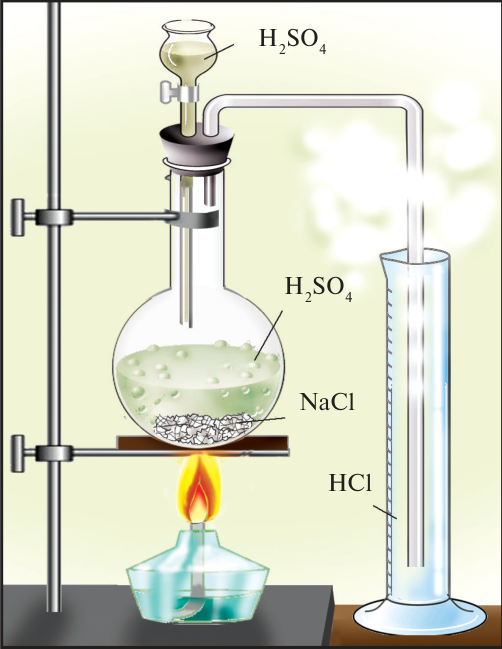
\includegraphics[width=0.86\linewidth]{rasmlar/darslik/d_hcl_lab.png}\end{center}
\noindent A)~\textsl{uchuvchan bo`lmagan kuchli kislota sifatida HCl ni siqib chiqaradi}\par
\noindent B)~\textsl{reaksiyada ishtirok etmaydi}\par
\noindent C)~\textsl{tuzni oksidlaydi}\par
\noindent D)~\textsl{faqat erituvchi vazifasini bajaradi   ---}\par
\vspace{4pt}
\end{multicols}
\medskip
\noindent\setlength{\fboxsep}{0pt}\fbox{\begin{tabular}{p{0.74\linewidth}|p{0.2\linewidth}}
\parbox[t]{0.72\linewidth}{\vspace{3pt}\textbf{Topshiriqlar (33--35) va javob variant (A--F)larini o`zaro to`g`ri moslashtiring.} Mis va magniy (Cu va Mg) dan iborat 26,4 g qotishma mo`l H\textsubscript{2}SO\textsubscript{4} eritmasida eritilganda 6,72 l (n.sh.) gaz ajraldi (mis kislota bilan reaksiyaga kirishmaydi).
\vspace{3pt}} & \parbox[t]{0.19\linewidth}{\vspace{3pt}A~\textsl{147}\\[3pt]
B~\textsl{72,73}\\[3pt]
C~\textsl{220,5}\\[3pt]
D~\textsl{109,09}\\[3pt]
E~\textsl{36,36}\\[3pt]
F~\textsl{36}}\\ \hline
\parbox[t]{0.72\linewidth}{\vspace{2pt}\textbf{33. Qotishmadagi Cu massa ulushini (\%) aniqlang.}\vspace{2pt}} & \\ \hline
\parbox[t]{0.72\linewidth}{\vspace{2pt}\textbf{34. Reaksiya uchun sarflangan 20\% li H\textsubscript{2}SO\textsubscript{4} massasini (g) aniqlang.}\vspace{2pt}} & \\ \hline
\parbox[t]{0.72\linewidth}{\vspace{2pt}\textbf{35. Eritmadagi tuzlarning umumiy massasini (g) aniqlang.}\vspace{2pt}} & 
\end{tabular}}
\par\bigskip
\noindent\textbf{36.} Cu + H\textsubscript{2}SO\textsubscript{4} $\to$ CuSO\textsubscript{4} + SO\textsubscript{2} + H\textsubscript{2}O reaksiya tenglamasini elektron balans usulida tenglang va barcha koeffitsiyentlar \textbf{yig`indisini aniqlang.}
\javob
\noindent\textbf{37.} CuSO\textsubscript{4} eritmasi inert elektrodlar yordamida 2 A tok kuchi bilan 965 s elektroliz qilindi. Anodda ajralgan O\textsubscript{2} hajmi (l, n.sh.) \textbf{ni toping.}
\javob
\noindent\textbf{38.} Alyuminiy va rux dan iborat 9,2 g aralashma mo`l xlorid kislotada eritilganda 5,6 l (n.sh.) vodorod ajraldi. Aralashmadagi alyuminiyning massa \textbf{ulushini (\%) aniqlang.}
\javob
\noindent\textbf{39.} Etilen va asetilendan iborat 4,48 l (n.sh.) aralashma bromli suvdan o`tkazilganda 48 g brom yutildi. Aralashmadagi asetilenning \textbf{hajmini (l, n.sh.) toping.}
\javob
\noindent\textbf{40.} Polimerlanish darajasi 2000 bo`lgan polietilen ning 280 g namunasini olish uchun polimerlanish unumi 80\% bo`lganda qancha monomer (C\textsubscript{2}H\textsubscript{4}) kerak (g)?
\javob
\par\bigskip\begin{center}\textbf{\fontsize{13}{15}\selectfont YOZMA ISH}\end{center}
\noindent\textbf{41.} \textbf{Topshiriqni bajarish jarayonida barcha reaksiya tenglamalarini yozing. Miqdoriy va arifmetik hisoblashlarni (unga asos bo`lgan usul yoki formulani ko`rsatgan holda) uzviy ketma-ketlikda bajaring.}\par\smallskip
CO va CO\textsubscript{2} dan iborat gazlar aralashmasi (n.sh.) 5,6 l hajm egallaydi va massasi 7,8 g.\par
\noindent 1)Aralashmadagi gazlarning mol miqdorlarini hisoblang.\par
\noindent 2)Aralashmaning vodorodga nisbatan zichligini va gazlarning hajmiy ulushlarini (\%) aniqlang. Aralashmaning to`liq massasini (g) ham ayting.\par
\noindent 3)Aralashmani to`liq yoqish uchun zarur kislorod hajmini (l, n.sh.) toping.\par
\noindent 4)Yonishdan keyingi gazlar mo`l NaOH eritmasidan o`tkazildi. Hosil bo`lgan Na\textsubscript{2}CO\textsubscript{3} massasini (g) hisoblang (CO\textsubscript{2} + 2NaOH $\to$ Na\textsubscript{2}CO\textsubscript{3} + H\textsubscript{2}O). NaOH sarfini (g) ham toping (CO\textsubscript{2} + 2NaOH $\to$ Na\textsubscript{2}CO\textsubscript{3} + H\textsubscript{2}O).\par
\noindent 5)Aralashmaning o`rtacha molyar massasini (g/mol) toping. Shu miqdor CO ni yoqish uchun havo (21\% O\textsubscript{2}) hajmi qancha (l, n.sh.)?\par
\diqqat{Mazkur topshiriq kengaytirilgan javobni talab etib, uning yechilish usuli va shu usul asosidagi barcha hisoblash amallari javoblar varaqasida aks etishi lozim.}
\noindent\textbf{42.} Quyidagi o`zgarishlar zanjirida \textit{X}, \textit{Y}, \textit{Z} noma'lum organik moddalar:\par
\[\setlength{\fboxsep}{0pt}\text{CH\textsubscript{4}}\xrightarrow{\text{Cl\textsubscript{2}, yorug`lik}}\text{\textit{X}}\xrightarrow{\text{Na}}\text{\textit{Y}}\xrightarrow{\text{Cl\textsubscript{2}, yorug`lik}}\text{\textit{Z}}\xrightarrow{\text{KOH (suvli)}}\text{C\textsubscript{2}H\textsubscript{5}OH}\]
\noindent 1)CH\textsubscript{4} $\to$ \textit{X} : reaksiya tenglamasini yozing; hosil bo`lgan moddani nomlang.\par
\noindent 2)\textit{X} $\to$ \textit{Y} : reaksiya tenglamasini yozing; hosil bo`lgan moddani nomlang.\par
\noindent 3)\textit{Y} $\to$ \textit{Z} : reaksiya tenglamasini yozing; hosil bo`lgan moddani nomlang.\par
\noindent 4)\textit{Z} $\to$ C\textsubscript{2}H\textsubscript{5}OH : reaksiya tenglamasini yozing; hosil bo`lgan moddani nomlang.\par
\diqqat{Mazkur topshiriq kengaytirilgan javobni talab etib, uning yechilish usuli va shu usul asosidagi barcha hisoblash amallari javoblar varaqasida aks etishi lozim.}
\noindent\textbf{43.} \textbf{Topshiriqni bajarish jarayonida barcha reaksiya tenglamalarini yozing. Miqdoriy va arifmetik hisoblashlarni (unga asos bo`lgan usul yoki formulani ko`rsatgan holda) uzviy ketma-ketlikda bajaring.}\par\smallskip
Magniy (Mg) va rux (Zn) dan iborat 8,9 g qotishma mo`l suyultirilgan sulfat kislotada eritildi, bunda 4,48 l (n.sh.) gaz ajraldi. Hosil bo`lgan eritmaga mo`l NaOH eritmasi qo`shildi, hosil bo`lgan cho`kma ajratib olindi va havoda qizdirib quritildi.\par
\noindent 1)Reaksiya tenglamalarini yozing va qotishmadagi har bir metallning massasini (g) aniqlang.\par
\noindent 2)Qotishmadagi Mg ning massa ulushini (\%) hisoblang.\par
\noindent 3)Eritish uchun sarflangan 20\% li H\textsubscript{2}SO\textsubscript{4} eritmasining massasini (g) aniqlang.\par
\noindent 4)Mo`l NaOH qo`shilganda hosil bo`lgan cho`kmaning formulasi va massasini (g) toping (reaksiya tenglamalarini yozing).\par
\noindent 5)Cho`kma havoda to`liq qizdirilganda hosil bo`lgan oksidning massasini (g) hisoblang.\par
\diqqat{Mazkur topshiriq kengaytirilgan javobni talab etib, uning yechilish usuli va shu usul asosidagi barcha hisoblash amallari javoblar varaqasida aks etishi lozim.}
\newpage
\noindent\textbf{\fontsize{13}{15}\selectfont Nazorat testi}\ \textit{$\cdot$ 13-variant}\hfill \textbf{Javoblar kaliti}\par\smallskip\hrule\smallskip
\textit{Faqat o`qituvchi uchun.}\par\medskip
\noindent\textbf{1--32-savollar}\par\smallskip
\noindent\begin{tabular}{|c|c|c|c|c|c|c|c|c|c|c|c|c|c|c|c|}\hline
\textbf{1} & \textbf{2} & \textbf{3} & \textbf{4} & \textbf{5} & \textbf{6} & \textbf{7} & \textbf{8} & \textbf{9} & \textbf{10} & \textbf{11} & \textbf{12} & \textbf{13} & \textbf{14} & \textbf{15} & \textbf{16}\\\hline
\textsl{A} & \textsl{B} & \textsl{C} & \textsl{B} & \textsl{C} & \textsl{A} & \textsl{D} & \textsl{A} & \textsl{C} & \textsl{A} & \textsl{D} & \textsl{A} & \textsl{C} & \textsl{D} & \textsl{B} & \textsl{D}\\\hline
\textbf{17} & \textbf{18} & \textbf{19} & \textbf{20} & \textbf{21} & \textbf{22} & \textbf{23} & \textbf{24} & \textbf{25} & \textbf{26} & \textbf{27} & \textbf{28} & \textbf{29} & \textbf{30} & \textbf{31} & \textbf{32}\\\hline
\textsl{C} & \textsl{B} & \textsl{B} & \textsl{C} & \textsl{B} & \textsl{D} & \textsl{A} & \textsl{B} & \textsl{A} & \textsl{D} & \textsl{C} & \textsl{C} & \textsl{B} & \textsl{D} & \textsl{D} & \textsl{A}\\\hline
\end{tabular}\par\medskip
\noindent\textbf{33--35-savollar}\par\smallskip
\noindent\begin{tabular}{|c|c|c|}\hline \textbf{No} & \textbf{Javob} & \textbf{Qiymat}\\\hline
33 & \textsl{B} & 72,73\\\hline
34 & \textsl{A} & 147\\\hline
35 & \textsl{F} & 36\\\hline
\end{tabular}\par\medskip
\noindent\textbf{36--40-savollar}\par\smallskip
\noindent\begin{tabular}{|c|c|}\hline \textbf{No} & \textbf{To`g`ri javob}\\\hline
36 & 7\\\hline
37 & 0,112\\\hline
38 & 29,3\\\hline
39 & 2,24\\\hline
40 & 350\\\hline
\end{tabular}\par\medskip
\noindent\textbf{41--43-topshiriqlar: qisqa yechim}\par\smallskip
\noindent\textbf{41-topshiriq.}\par
\noindent 1) x + y = 0,25; 28x + 44y = 7,8 $\to$ n(CO) = \textbf{0,2 mol}, n(CO\textsubscript{2}) = \textbf{0,05 mol}\par
\noindent 2) M = 31,2; D(H\textsubscript{2}) = \textbf{15,6}; $\varphi$(CO) = 80\%, $\varphi$(CO\textsubscript{2}) = 20\%; m = \textbf{7,8 g}\par
\noindent 3) 2CO + O\textsubscript{2} $\to$ 2CO\textsubscript{2}: 0,2 mol $\cdot$ 0,5 $\cdot$ 22,4 = \textbf{2,24 l}\par
\noindent 4) CO\textsubscript{2} jami = 0,25 mol $\to$ Na\textsubscript{2}CO\textsubscript{3} = 0,25 mol = \textbf{26,5 g}; m(NaOH) = 2$\cdot$0,25$\cdot$40 = \textbf{20 g}\par
\noindent 5) M(o`rt.) = m/n = \textbf{31,2 g/mol}; \textit{V}(havo) = 2,24/0,21 = \textbf{10,67 l}\par
\noindent Jami: M 15 + A 10 = 25 ball.\par
\noindent\textbf{42-topshiriq.}\par
\noindent 1) CH\textsubscript{4} + Cl\textsubscript{2}, yorug`lik $\to$ CH\textsubscript{3}Cl (xlormetan)\par
\noindent 2) CH\textsubscript{3}Cl + Na $\to$ C\textsubscript{2}H\textsubscript{6} (etan)\par
\noindent 3) C\textsubscript{2}H\textsubscript{6} + Cl\textsubscript{2}, yorug`lik $\to$ C\textsubscript{2}H\textsubscript{5}Cl (xloretan)\par
\noindent 4) C\textsubscript{2}H\textsubscript{5}Cl + KOH (suvli) $\to$ C\textsubscript{2}H\textsubscript{5}OH (etanol)\par
\noindent Jami 25 ball.\par
\noindent\textbf{43-topshiriq.}\par
\noindent 1) x$\cdot$24 + y$\cdot$65 = 8,9; 1 x + 1 y = 0,2 mol $\to$ n(Mg) = 0,1 mol (\textbf{2,4 g}), n(Zn) = 0,1 mol (\textbf{6,5 g})\par
\noindent 2) $\omega$(Mg) = 2,4/8,9 = \textbf{27\%}\par
\noindent 3) n(H\textsubscript{2}SO\textsubscript{4}) = n(H\textsubscript{2}) = 0,2 mol = 19,6 g; eritma: 19,6/0,2 = \textbf{98 g}\par
\noindent 4) Mo`l NaOH da Zn(OH)\textsubscript{2} amfoter bo`lgani uchun eriydi; cho`kma Mg(OH)\textsubscript{2}: 0,1 mol $\cdot$ 58 = \textbf{5,8 g}\par
\noindent 5) Mg(OH)\textsubscript{2} $\to$ MgO + H\textsubscript{2}O: 0,1 mol $\cdot$ 40 = \textbf{4 g}\par
\noindent Jami: M 15 + A 10 = 25 ball.\par
\par\bigskip\noindent\textbf{Mavzular taqsimoti}\par\smallskip
{\small\noindent\begin{longtable}{|c|p{7.2cm}|p{5.4cm}|c|}\hline \textbf{No} & \textbf{Mavzu} & \textbf{Tekshiriladigan ko`nikma} & \textbf{Ball}\\\hline
1 & Tirkashev VI bob (muvozanat, jadval) & Jadval tahlili & 1\\\hline
2 & Tirkashev VI bob (muvozanat, jadval) & Jadval tahlili & 1\\\hline
3 & Tirkashev VI bob (kimyoviy muvozanat) & Hisoblash va masala yechish & 1\\\hline
4 & Tashev; 9-sinf (kuchlanish qatori) & Bilim va tushunish & 1\\\hline
5 & 11-sinf (Mendeleyev--Klapeyron) & Hisoblash va masala yechish & 1\\\hline
6 & 11-sinf 8-bob (Faradey qonunlari); Tirkashev \textit{V} bob & Hisoblash va masala yechish & 1\\\hline
7 & 8-sinf (ionlanish energiyasi, grafik) & Grafik tahlili & 1\\\hline
8 & 9-sinf (gidroliz); Tirkashev IV bob & Bilim va tushunish & 1\\\hline
9 & 11-sinf 4-bob (molyar konsentratsiya) & Hisoblash va masala yechish & 1\\\hline
10 & 11-sinf (ekvivalentlar qonuni) & Hisoblash va masala yechish & 1\\\hline
11 & 10-sinf \S{}17 (gibridlanish); Abdusamatov & Bilim va tushunish & 1\\\hline
12 & 11-sinf 8-bob; Tirkashev \textit{V} bob (elektroliz) & Bilim va tushunish & 1\\\hline
13 & Tirkashev I bob; 8-sinf (elektron konfiguratsiya) & Bilim va tushunish & 1\\\hline
14 & 9-sinf; Tirkashev (P/C/Si, hisob) & Hisoblash va masala yechish & 1\\\hline
15 & 9-sinf; Tirkashev (galogenlar, hisob) & Hisoblash va masala yechish & 1\\\hline
16 & 9-sinf (ishqoriy metallar); Tashev & Bilim va tushunish & 1\\\hline
17 & 9-sinf (alyuminiy) & Hisoblash va masala yechish & 1\\\hline
18 & 9-sinf; Tashev (Fe, Cu, Zn, Cr) & Bilim va tushunish & 1\\\hline
19 & 9-sinf; Tirkashev (suv qattiqligi, hisob) & Hisoblash va masala yechish & 1\\\hline
20 & 10-sinf (mavzuga oid paragraflar); Abdusamatov & Bilim va tushunish & 1\\\hline
21 & 10-sinf \S{}13, \S{}15 (alken va alkin birikish reaksiyalari) & Hisoblash va masala yechish & 1\\\hline
22 & 10-sinf (ikki bosqichli hisob) & Hisoblash va masala yechish & 1\\\hline
23 & 10-sinf (gibridlanish) & Rasm bo`yicha tahlil & 1\\\hline
24 & 10-sinf (ikki bosqichli hisob) & Hisoblash va masala yechish & 1\\\hline
25 & 10-sinf \S{}26 & Hisoblash va masala yechish & 1\\\hline
26 & 10-sinf (ikki bosqichli hisob) & Hisoblash va masala yechish & 1\\\hline
27 & 10-sinf \S{}30--31 (bijg`ish) & Hisoblash va masala yechish & 1\\\hline
28 & 10-sinf (organik birikmalar sinflari) & Bilim va tushunish & 1\\\hline
29 & 10-sinf \S{}35 (YuMB) & Hisoblash va masala yechish & 1\\\hline
30 & 7-sinf (xavfsizlik qoidalari); 10-sinf lab. & Bilim va tushunish & 1\\\hline
31 & 7-sinf (aralashmalarni ajratish usullari) & Bilim va tushunish & 1\\\hline
32 & 8-sinf (17-rasm) & Rasm bo`yicha tahlil & 1\\\hline
33--35 & Aralash masala (moslashtirish) & Ko`p bosqichli hisob & 3\\\hline
36--40 & Qisqa javobli masalalar & Hisoblash & 5\\\hline
41--43 & Yozma ish & Usul va hisob (M, A) & 75\\\hline
\end{longtable}}
\end{document}
